\documentclass[11pt]{article}
\usepackage{amssymb, amsmath,amsthm,enumitem,multirow,hhline,bbm,mathtools, pythonhighlight,comment, float,grffile,tikz}
\usepackage{pdfpages,pgfplots}
\usepackage{graphicx, setspace}
\usepackage{enumitem, hyperref, varwidth}
\usepackage[a4paper, total={5in, 8in}]{geometry}
\usetikzlibrary{matrix}
\setlength\parindent{0pt}
\newcommand{\forceindent}{\leavevmode{\parindent=1.5em\indent}}
\newcommand{\iidsim}{\stackrel{\mathclap{iid}}{\sim}}
\newcommand{\mathsym}[1]{{}}
\newcommand{\unicode}[1]{{}}

\newcounter{mathematicapage}
\allowdisplaybreaks
\author{Rick Shen}
\begin{document}
\begin{center}
    \vspace*{\fill}
        \Large\textbf{Homework 1}\\
        \Large\text{628 Machine Learning in Finance}\\    
        \large\textit{Rick Shen}\\
        \large\textit{Fall 2024}
    \vspace*{\fill}
\end{center}

\includepdf[pages=-]{Homework week 1}
The code appears to do the following:
\begin{enumerate}
    \item It loads the `MNIST' dataset, which contains a training set of $60000$ samples, each with a $78 \times 78$ pixle image of an integer number between $0$ to $9$.
    \item The dataset also contains a testing set of size $10000$, which is used to test the model. 
    \item It chooses the number $8$, and aim to use logistic regression technique to tell if an image displays that number. 
    \item It uses several criterial to assess the model's goodness of fit such as ROC curve.
    \item Towards the end, it uses advanced techniques such as ensemble modeling. 
\end{enumerate}
\begin{figure}
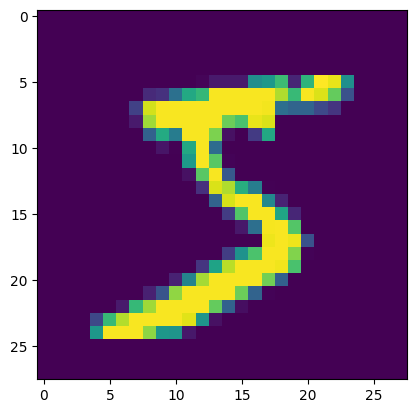
\includegraphics{output.png}[h]
\caption{The first image from the training set}
\end{figure}
When I first ran the code as-is, I'd get a warning message. 

\begin{python}
    from sklearn.linear_model import LogisticRegression

    model = LogisticRegression(random_state=0, solver='lbfgs')

/usr/local/lib/python3.7/dist-packages/sklearn/linear_model/_logistic.py:940: ConvergenceWarning: lbfgs failed to converge (status=1):
STOP: TOTAL NO. of ITERATIONS REACHED LIMIT.
\end{python}
\vspace{1em}  
It appears as if the regression did not converge. \\
Upon reading the document from Scikit-Learn, I had learned that scaling the predictors can improve the performance 
of the regression model. So I modified the code by normalizing the X values.
\vspace{1em}  
\begin{python}
from sklearn.linear_model import LogisticRegression
from sklearn.preprocessing import StandardScaler

scaler = StandardScaler()
X_train_scaled = scaler.fit_transform(X_train)  # normalize X values from training set
X_test_scaled = scaler.transform(X_test)    # normalize X values from testing set

model = LogisticRegression(random_state=0, solver='lbfgs')
clf = model.fit(X_train_scaled, Y_train)

# Predict labels
y_train_est = clf.predict(X_train_scaled)
y_train_prob_est = clf.predict_proba(X_train_scaled)

# Predict probabilities
y_test_est = clf.predict(X_test_scaled)
y_test_prob_est = clf.predict_proba(X_test_scaled)
\end{python}
\vspace{1em}    
By doing so, no only did the warning message disappeared, the ROC-AUC value also increased slightly, indicating 
that indeed scaling the predictor can improve performance. 
\begin{figure}
    \includegraphics*{ROC_orig.png}
    \caption{Area under the curve before scaling}
    \includegraphics*{ROC_scaled.png}
    \caption{Area under the curve after scaling}
\end{figure}
% \textbf{Problem 1.} \\[6pt]
% 1.\\
% $$f^\prime (t) = \frac{f(t)}{1-t} +1 , \hspace{6pt} t\in (0,1), \hspace{6pt} f(1)=0.$$
% Prove that $f(t)= -\frac{1}{2} (1-t)$ solve the ODE.
% \begin{proof}
% \begin{align*}
%     f^\prime (t) & =-\frac{1}{2}(1-t)^\prime = \frac{1}{2}\\
%     & = \frac{-\frac{1}{2}(1-t)}{1-t}+1= \frac{f(t)}{1-t}+1 
% \end{align*}
% \end{proof}
% Try to solve starting from $t=1$ going backward.\\
% Euler's explicit method:
% \begin{align*}
%     \frac{(f(t_n) - f(t_{n-1}))}{dt} &= \frac{f(t_n)}{1- (n-1) dt} + 1 \\
%     % \frac{(f(t_n) - f(t_{n-1}))}{dt} &= \frac{f(t_n)}{1- (n-1) dt} + 1 \\
%     \Rightarrow f(t_{n-1}) & = f(t_n) - \left( \frac{f(t_n)}{1-(n-1)dt}+1\right) dt\\
%     % f(t_{n-1}) & = f(t_n) -\left( \frac{f(t_n)}{t_{n-1}}+1\right) dt\\
% \end{align*}
% Euler's implicit method:
% \begin{align*}
%     \frac{(f(t_n) - f(t_{n-1}))}{dt} &= \frac{f(t_{n-1})}{1- (n-1) dt} + 1 \\
%     \Rightarrow f(t_{n-1}) & = (f(t_n)-dt)\left( 1+\frac{dt}{1-(n-1) dt}\right)
% \end{align*}
% Try to solve starting from $t=0$ going forward.\\
% Euler's implicit method:
% \begin{align*}
%     \frac{f(t_{n+1}-f(t_n))}{dt} & = \frac{f(t_{n+1})}{1-ndt} + 1 \\
%     \Rightarrow f(t_{n+1}) & = (f(t_n)+dt)\left(1- \frac{1}{1-ndt}\right)
% \end{align*}
% See code and output next page. Both explicit and implicit methods work well 
% when solving backward from $t=1$. However, when done forward from $t=0$, the
% implicit method becomes unstable as $t \to 1$. A look at the solution for $f(t_{n+1})$
% reveals that the denominator $1-ndt$ becomes large which leads to the error.
% \includepdf[pages=-]{Problem_1}
% \textbf{Problem 2.}
% \begin{align*}
%     g(t,y) &:= f\left(T-t,e^{\frac{1}{\sqrt{2}} \sigma y - \frac{1}{2}\sigma^2 (T-t)}\right)\\
%     x &:= e^{\frac{1}{\sqrt{2}} \sigma y - \frac{1}{2} \sigma^2(T-t)}\\
%     \Rightarrow \frac{\partial x}{\partial y} & = \frac{1}{\sqrt{2}} \sigma x\\
%     \frac{\partial x}{\partial t} & = \frac{1}{2} \sigma^2\\
%     g(t,y) &:= f\left(T-t, e^{\frac{1}{\sqrt{2}} \sigma y - \frac{1}{2} \sigma^2(T-t)}\right)\\
%     \Rightarrow g_t := \frac{\partial g}{\partial t} & = - f_t + \frac{\partial f}{\partial x} \frac{\partial x}{\partial t} = -f_t + \frac{1}{2}\sigma^2 x f_x\\
%     \Rightarrow f_t &= \frac{1}{2} \sigma^2 x f_x - g_t\\
%     g_y := \frac{\partial g}{\partial y} & = \frac{\partial f}{\partial x} \frac{\partial x}{\partial y} = f_x \frac{1}{\sqrt{2}}\sigma x\\
%     g_{yy} := \frac{\partial^2 g}{\partial y^2 } & = 
%     \frac{\partial }{\partial x} \left( f_x \frac{1}{\sqrt{2}} \sigma x \right) \frac{\partial x}{\partial y} 
%     = \left(f_{xx} \frac{1}{\sqrt{2}} \sigma x + \frac{1}{\sqrt{2}} \sigma f_x \right) \frac{1}{\sqrt{2}}\sigma x\\
%     &= \frac{1}{2} \sigma^2 x^2 f_{xx} + \frac{1}{2} \sigma^2 x f_x \\
%     \Rightarrow \frac{1}{2} \sigma^2 x^2 f_{xx}  & = g_{yy} - \frac{1}{2} \sigma^2 xf_x
% \end{align*}
% Plug in the Black-Scholes PDE, the $f_x$ terms canceled out, we'd get
% \begin{align*}
%     \left\{ \begin{array}{ll}
%     g_t = g_{yy} \\
%     g(y,0) = F \left(e^{\frac{1}{\sqrt{2}} \sigma y - \frac{1}{2}\sigma^2 T} \right)
%     \end{array} \right.
% \end{align*}
% which is the PDE that $g(t,y)$ would satisfy.\\[9pt]
% \textbf{Problem 3.}\\[6pt]
% Under the Black-Scholes frame work, and assume $r=0$, the PDE is 
% \begin{align*}
%         \left\{ \begin{array}{ll}
%         f_t(x,t) = \frac{1}{2} \sigma^2 x^2 f_{xx}\\
%         f(x,0) = (K-x)^+ 
%     \end{array} \right.
% \end{align*}
% Where $f(x, T-t)$ is the value of the option at time $T-t$ and stock price $x:=S_t$. 
% % Use the result in \textbf{Problem 2.}, Let
% % $$ u(x, t) = f(T-t, e^{ \sigma y - \frac{1}{2}\sigma^2(T-t)})$$
% % satisfies the PDE
% % \begin{align*}
% %     \left\{ \begin{array}{ll}
% %         u_t(x,t) = \frac{1}{2} \sigma^2 u_{xx}\\
% %         u(x,0) = (K-x)^+ 
% %     \end{array} \right.
% % \end{align*}
% % % Note that this implies $y = \sqrt{2} B_t $ in the Black-Scholes framework, where $x$ is taken to be the stock price $S_t$ at time $t$.\\
% % Under the Black-Scholes framework, this means $x = S_t$ and $y=B_t$ at time $t$.\\
% In addition to the initial condition, for the European put option, the parabolic boundary conditions are
% \begin{align*}
%     \left\{ \begin{array}{ll}
%         f(\underbrace{0}_{xL}, t) = K\\
%         f(\underbrace{\infty}_{xH}, t) = 0 
%     \end{array} \right.
% \end{align*}
% Crank-Nicolson method for the system described is
% $$\left(\mathbf{I} - \frac{1}{4} \alpha \mathbf{X} \mathbf{C}\right) \vec{u}^{m+1} =\left(\mathbf{I} +\frac{1}{4} \alpha \mathbf{X} \mathbf{C}\right) \vec{u}^m + \frac{\alpha}{2} \vec{u}_L + \frac{\alpha}{2} \vec{u}_H$$
% where $\mathbf{I},\,\mathbf{X},\, \mathbf{C} \in \mathbb{R}^{N \times N}$, and all $\vec{u} \in \mathbb{R}^N$.
% \begin{align*}
%     \mathbf{X}  = \begin{pmatrix}
%         x^2_1& 0& 0 & \ldots & 0\\
%         0 & x^2_2 & 0 & \ldots & 0\\
%         \vdots & &\ddots& &\vdots\\
%         0 & \ldots & & 0& x^2_N
%     \end{pmatrix},
%     \hspace{6pt}
%     \mathbf{C}  = \begin{pmatrix}
%         -2& 1& 0 & \ldots & 0\\
%         1 & -2 & 1 & \ldots & 0\\
%         \vdots & &\ddots& &\vdots\\
%         0 & \ldots & & 1& -2
%     \end{pmatrix},\\
%     % \hspace{6pt}
%     \vec{u}_L = \begin{pmatrix}
%         U_L(t_m) + U_L(t_{m+1})\\
%         0\\
%         \vdots\\
%         0
%     \end{pmatrix},
%     \hspace{6pt}
%     \vec{u}_H = \begin{pmatrix}
%         0\\
%         \vdots\\
%         0\\
%         U_H(t_m) + U_H(t_{m+1})
%     \end{pmatrix}
% \end{align*}
% \includepdf[pages=-]{Problem_3}
\end{document} 